\section{The arithmetic question and the result}
The preceding receiver calculation isolates a polynomial $F$ governing the
original sign-odd receiving matrix of a quartic factor-inverse construction
\cite[EZ37--EZ45]{Receiver}. A later audit proves nonvanishing on a
three-character prime locus and also constructs positive real and $p$-adic
zeros outside the integral locus. We use its literal polynomial, roots, signs
and coefficient normalization, read directly in the pinned public continuation
\cite[Track I, E1--E6]{Frame}. The present
result settles its integral nonvanishing question; it does not assert the
existence of an Erd\H{o}s--Straus (ES) witness at every prime.

\begin{theorem}[Global arithmetic receiving determinant]\label{thm:main}
Let $p\equiv1\pmod{12}$ be prime and let $x,y,z$ be positive integers satisfying
$4/p=1/x+1/y+1/z$. Retain the four literal roots
$\ell=(p,x,y,z)$ and put
\[
 S=p+x+y+z,\qquad
 H(T)=-S^{-1}\prod_{i=0}^3(T-\ell_i)=AT^4+T^3+BT^2+CT+D.
\]
Define $F$ by \eqref{eq:F} and $\mathfrak N=S^6F$. Then $\mathfrak N$ is an
integer and
\begin{equation}\label{eq:main}
 \boxed{\mathfrak N<-c_{12}p^8<0,\qquad
 c_{12}=\frac{125873811}{262144}.}
\end{equation}
If $p\equiv1\pmod{24}$, one may replace $c_{12}$ by
\begin{equation}\label{eq:c24}
 \boxed{c_{24}=\frac{327448292668}{47045881}.}
\end{equation}
For the original odd receiving matrix $O$, every retained choice of root order
and square-root signs gives
\[
 |\det O|>\frac{4c\,p^8}{S^3},\qquad
 \|O^{-1}\|_2<\frac{360}{c}\frac{S^9}{p^8},
\]
where $c$ is the applicable constant. These constants are not asserted optimal
on the original integral witness domain.
\end{theorem}
The proof uses two finite, universal polynomial coefficient identities. The
complete integer arrays and two separate standard-library checks are supplied.
The arithmetic census is a corroboration of the implementation, not the
proof of the universal coefficient identities or the theorem.

\section{Original states and the complete first-half domain}
Here we give the elementary reductions needed to apply the theorem to every
witness, rather than assume that its distinguished denominator has been chosen
in a restricted family. The Type I/II framework is classical
\cite[\S2, Propositions 2.2 and 2.6]{ET}.

Every denominator exceeds $p/4$. At least one is divisible by $p$, by clearing
the reciprocal equation; all three cannot be, since their reciprocal sum
would then be at most $3/p$. A denominator equal to $p$ would give
\[
 (3y-p)(3z-p)=p^2.
\]
Here $y,z>p/3$, so both displayed factors are positive. The positive factors
of $p^2$ are $1\pmod3$, whereas each displayed factor is $2\pmod3$. Hence no
denominator equals $p$. If two denominators equal $a$, positivity of the third
denominator gives $d=2a-p>0$. Then $4dz=p(d+p)$ and $d\mid p^2$. The three possibilities
$d=1,p,p^2$ give respectively $z=p(p+1)/4,p/2,(p+1)/4$, all nonintegral for
$p\equiv1\pmod4$. Thus all four literal roots are distinct.

If two denominators are multiples of $p$, the third, denoted by $a$, must satisfy
$a<p/2$: otherwise the sum is at most $4/p$, with equality requiring the
impossible integer $a=p/2$. The other two denominators exceed $a$.

If exactly one denominator is $pk$, let the other two be $a\le b$, both units
at $p$. The identity
\[
 (4k-1)ab=pk(a+b)
\]
gives $4k-1=pt$, where $t\equiv3\pmod4$ and $\gcd(k,t)=1$. Write
$a=gr,b=gs$, $r\le s$, $\gcd(r,s)=1$. Then $tgrs=k(r+s)$, so $k=drs$,
$r+s=t\lambda$ and $g=d\lambda$: indeed $\gcd(rs,r+s)=1$ gives
$rs\mid k$, say $k=drs$; then $tg=d(r+s)$, and $\gcd(d,t)=1$ gives the
remaining two divisibilities. If $a\ge p/2$, substitution of
$p=(4drs-1)/t$ and $a=d\lambda r$ gives
\[
 2dr(r-s)\ge-1.
\]
The left side is an even nonpositive integer, forcing $r=s=1$ and $t\mid2$,
a contradiction. Thus again $p/4<a<p/2$, and $a$ is the unique smallest
original denominator.

Retain this $a$ and $R=4a-p$, so $3\le R<p$, $R\equiv3\pmod4$ and
$\gcd(pa,R)=1$. Since both tails exceed the unique smallest denominator, the
two factor coordinates
\[
 X=Ry-pa,qquad Z=Rz-pa
\]
are positive and satisfy
\[
 XZ=p^2a^2.
\]
Because $p\nmid R$, one has $p\mid X$ exactly when $p\mid y$, and likewise
for $Z,z$. Their $p$-valuation pairs are therefore $(0,2),(1,1),(2,0)$.
Place the unique $p$-divisible exterior denominator last. In the exterior and
oriented middle cases, respectively, there is a unique positive divisor
$u\mid a^2$ for which
\[
 E:\quad (X,Z)=(a^2/u,p^2u),qquad
 M:\quad (X,Z)=(pa^2/u,pu).
\]
Solving for the tails gives
\[
 E:\quad (y,z)=\left(\frac{pa+a^2/u}{R},\frac{pa+p^2u}{R}\right),
 \qquad
 M:\quad (y,z)=\left(\frac{p(a+a^2/u)}R,\frac{p(a+u)}R\right).
\]
Since $a,u,p$ are units modulo $R$ and $p\equiv4a\pmod R$, the two exact
integrality gates are
\begin{equation}\label{eq:gates}
 E:\ R\mid4u+1,\qquad M:\ R\mid a+u.
\end{equation}
Put
\[
 g=\gcd(a,u),\qquad(h,r,s)=(g^2/u,u/g,a/g).
\]
Primewise valuation gives $a=hrs,u=hr^2$, with all coordinates positive
integers and $\gcd(r,s)=1$. The ordered returns are
\begin{align}
 E:&\quad (a,hs\kappa,phr\kappa),&\kappa&=(pr+s)/R,\label{eq:E}\\
 M:&\quad (a,phs\lambda,phr\lambda),&\lambda&=(r+s)/R.\label{eq:M}
\end{align}
Their ordered inverses are $u=a^2/(Ry-pa)$ and $u=pa^2/(Ry-pa)$,
respectively. The middle complement $u\mapsto a^2/u$ exchanges $r,s$ and
only the last two denominators. Both orientations remain recorded. No
prime-factor exponents are identified across this map. The exterior case and
the two middle orientations exhaust every positive integral witness.

For E, the same rational identity exists even before the full gate:
\begin{equation}\label{eq:Eraw}
 (a,y,z)=\left(a,\frac{pa+a^2/u}{R},\frac{pa+p^2u}{R}\right).
\end{equation}
Every original E word has $u\ge2$, since $u=1$ would force $R\mid5$.
Moreover, write $(\cdot/R)$ for the Jacobi symbol and $(\cdot/p)$ for the
Legendre symbol. Then
\begin{equation}\label{eq:character}
 \left(\frac up\right)=-1.
\end{equation}
For an odd prime $q\mid a$, reciprocity and $R\equiv-p\pmod q$ give
\[
 \left(\frac qR\right)=(-1)^{(q-1)/2}\left(\frac Rq\right)
 =(-1)^{(q-1)/2}\left(\frac{-p}q\right)
 =\left(\frac pq\right)=\left(\frac qp\right).
\]
If $2\mid a$, the supplementary law and
$R\equiv-p\pmod8$ give the same identity at two. Multiplication yields
$({u}/{R})=({u}/{p})$, while the E gate gives
$u\equiv-4^{-1}\pmod R$. Hence $({u}/{R})=(-1/R)=-1$. This proves
\eqref{eq:character}. When $p\equiv1\pmod{24}$, two and three are residues,
so $u\ge5$. This character use is elementary and independent of the three
receiving-frame characters in the audit.

\section{The literal receiver and its integer determinant}
Let $e_i$ denote the elementary symmetric functions of the four literal roots.
Then
\[
 A=-1/S,\quad B=-e_2/S,\quad C=e_3/S,\quad D=-e_4/S.
\]
For $d_j=H'(\ell_j)$ choose and retain each sign
$\xi_j\in\mathbb C^\times$ with $\xi_j^2d_j=1$. The source's odd column is
\[
 o_j=\xi_j\bigl(1,-i d_j,A d_j^2+2\ell_jd_j,
                    i(7\ell_j^2d_j-13d_j^2)\bigr)^T.
\]
The supplied polynomial is
\begin{align}\label{eq:F}
 F={}&20(3C-B^2)+A(87B^3-282BC-51D)\notag\\
 &+A^2(-28B^4+22B^2C+431C^2+204BD)\notag\\
 &+A^3(224B^2D-168BC^2-856CD)-448A^4D^2.
\end{align}
Define the signed product
\[
 \epsilon=A^2\prod_{i<j}(\ell_j-\ell_i)\prod_i\xi_i\in\{1,-1\}.
\]
Then, exactly,
\begin{equation}\label{eq:det}
 \det O=\frac{4\epsilon F}{A^3}
       =-\frac{4\epsilon\mathfrak N}{S^3}.
\end{equation}
For completeness, reduce $1,H',A(H')^2+2TH',7T^2H'-13(H')^2$ modulo $H$ in
$1,T,T^2,T^3$. With the four row phases retained, the exact coefficient matrix
is $\mathsf C_H=\operatorname{diag}(1,-i,1,i)\mathsf M_H\in M_4(\mathbb C)$,
where
\[
\resizebox{\textwidth}{!}{$
\mathsf M_H=
\begin{pmatrix}
1&0&0&0\\
C&2B&3&4A\\
AC^2-9D&4ABC-8AD-7C&4AB^2-16A^2D-2AC-5B&4AB-8A^2C-3\\
20D/A-13C^2&20C/A+76D-52BC&20B/A+5C-52B^2+208AD&20/A-66B+104AC
\end{pmatrix}.$}
\]
Direct expansion gives $\det\mathsf M_H=4F/A$; the phases $-i,i$ have product
one. Evaluation at the roots and multiplication by the retained $\xi_j$ gives
\eqref{eq:det}, since
\[
 \prod_jd_j=A^4\prod_{i<j}(\ell_j-\ell_i)^2.
\]
The main verifier expands this complete Laurent-polynomial identity in
$A,B,C,D$, rather than testing selected targets.

The integer numerator, used without assuming $p\nmid S$, is
\begin{align}\label{eq:N}
\mathfrak N={}&60e_3S^5-20e_2^2S^4+87e_2^3S^2-282e_2e_3S^3-51e_4S^4\notag\\
&-28e_2^4+22e_2^2e_3S+431e_3^2S^2+204e_2e_4S^2\notag\\
&+224e_2^2e_4-168e_2e_3^2-856e_3e_4S-448e_4^2.
\end{align}
It is homogeneous of degree eight in the literal roots. Root permutation does
not change $\mathfrak N$, but the sign in \eqref{eq:det} is retained.

\begin{figure}[ht]
\centering
\resizebox{\textwidth}{!}{%
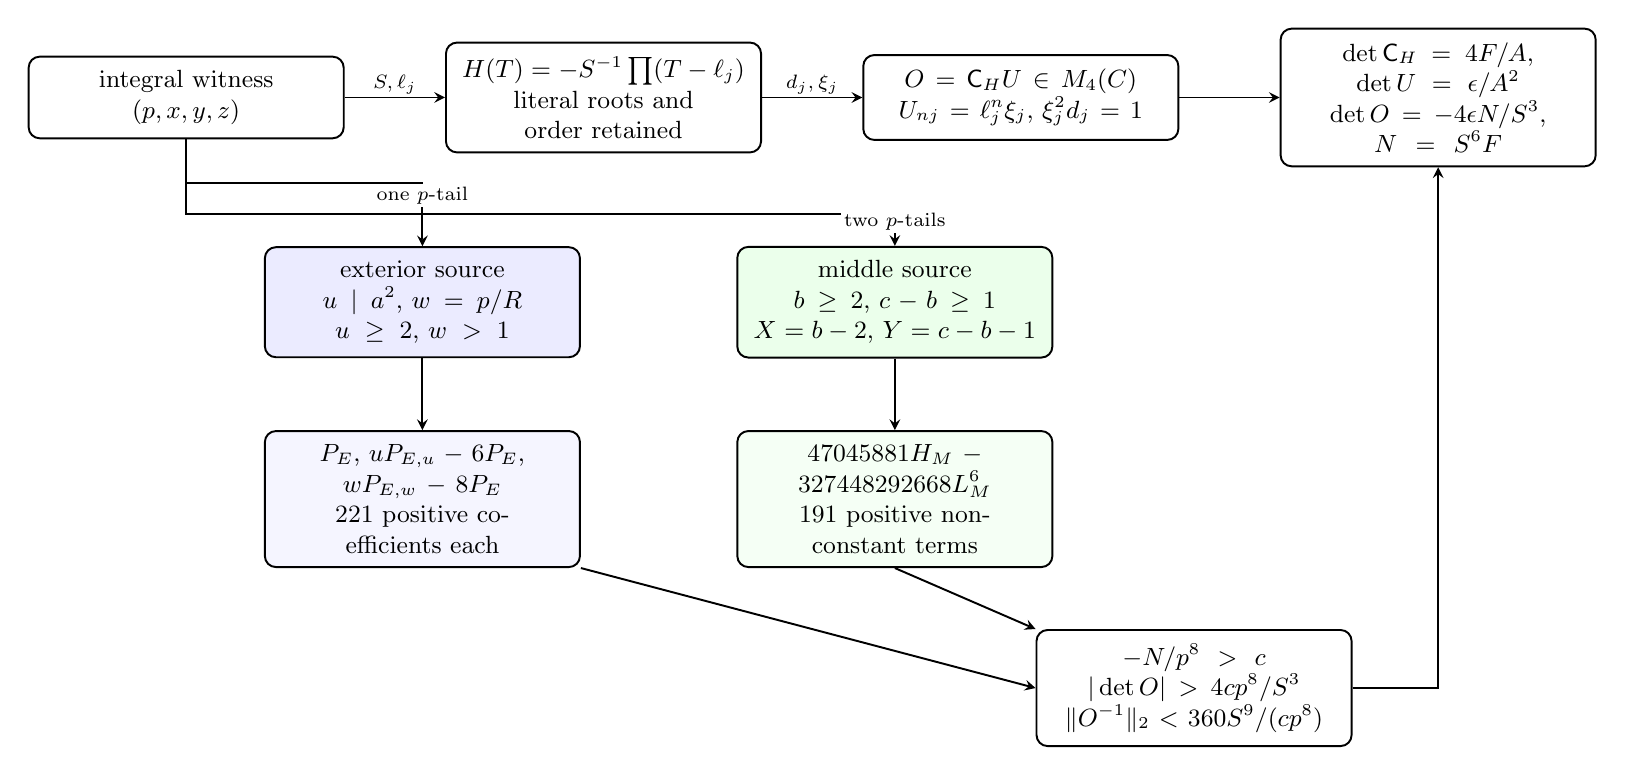
\begin{tikzpicture}[
  font=\small,>=stealth,
  box/.style={draw,rounded corners,align=center,inner sep=5pt,minimum height=1.0cm,text width=3.65cm},
  every path/.style={line width=.7pt}]
  \node[box] (w) at (0,0) {integral witness\\$(p,x,y,z)$};
  \node[box] (h) at (5.3,0) {$H(T)=-S^{-1}\prod(T-\ell_j)$\\literal roots and order retained};
  \node[box] (o) at (10.6,0) {$O=\mathsf C_HU\in M_4(\mathbb C)$\\$U_{nj}=\ell_j^n\xi_j$, $\xi_j^2d_j=1$};
  \node[box] (d) at (15.9,0) {$\det\mathsf C_H=4F/A$, $\det U=\epsilon/A^2$\\$\det O=-4\epsilon\mathfrak N/S^3$, $\mathfrak N=S^6F$};
  \draw[->] (w) -- node[above,font=\scriptsize,fill=white,inner sep=1pt] {$S,\ell_j$} (h);
  \draw[->] (h) -- node[above,font=\scriptsize,fill=white,inner sep=1pt] {$d_j,\xi_j$} (o);
  \draw[->] (o) -- (d);

  \node[box,fill=blue!8] (e) at (3.0,-2.6)
    {exterior source\\$u\mid a^2$, $w=p/R$\\$u\ge2$, $w>1$};
  \node[box,fill=green!8] (m) at (9.0,-2.6)
    {middle source\\$b\ge2$, $c-b\ge1$\\$X=b-2$, $Y=c-b-1$};
  \node[box,fill=blue!4] (ec) at (3.0,-5.1)
    {$P_E$, $uP_{E,u}-6P_E$, $wP_{E,w}-8P_E$\\$221$ positive coefficients each};
  \node[box,fill=green!4] (mc) at (9.0,-5.1)
    {$47045881H_M-327448292668L_M^6$\\$191$ positive nonconstant terms};
  \node[box] (c) at (12.8,-7.5)
    {$-\mathfrak N/p^8>c$\\$|\det O|>4cp^8/S^3$\\$\|O^{-1}\|_2<360S^9/(cp^8)$};
  \draw[->] (w.south) -- ++(0,-.55) -| node[pos=.70,above,font=\scriptsize,fill=white,inner sep=1pt] {one $p$-tail} (e.north);
  \draw[->] (w.south) -- ++(0,-.95) -| node[pos=.82,above,font=\scriptsize,fill=white,inner sep=1pt] {two $p$-tails} (m.north);
  \draw[->] (e) -- (ec);
  \draw[->] (m) -- (mc);
  \draw[->] (ec.south east) -- (c.west);
  \draw[->] (mc.south) -- (c.north west);
  \draw[->] (c.east) -| (d.south);
\end{tikzpicture}
}%
\caption{Typed route from a positive integral witness to the receiver bound.
The two arithmetic branches exhaust the witness domain.  The root labels,
square-root signs, complex coefficient map and determinant phase are retained;
the polynomial certificates control only the final real scalar
$-\mathfrak N/p^8$.}
\label{fig:determinant-mechanism}
\end{figure}


\section{Exterior arithmetic has a monotone positive certificate}
In \eqref{eq:Eraw} set $w=p/R>1$. Dividing the four roots by $p$ gives
\[
 \left(1,\frac{w+1}{4w},
 \frac{w+1}{4}+\frac{(w+1)^2}{16wu},\frac{w+1}{4}+wu\right).
\]
Define the exact polynomial $P_E$ by
\begin{equation}\label{eq:PEdef}
 \begin{split}
 -64u^2P_E(u,w)=\mathfrak N\bigl(&16wu,4u(w+1),\\
 &(w+1)(4wu+w+1),4wu(w+1+4wu)\bigr).
 \end{split}
\end{equation}
The right side is divisible by $64u^2$ in $\mathbb Z[u,w]$; the sign on the
left is part of the definition. The resulting bidegree is $(12,16)$. Hence
\begin{equation}\label{eq:QE}
 -\frac{\mathfrak N(p,a,y,z)}{p^8}
 =Q_E(u,w):=\frac{P_E(u,w)}{2^{26}u^6w^8}.
\end{equation}

\begin{lemma}[Finite universal exterior coefficient certificate]\label{lem:Epoly}
Each of
\[
 P_E(1+X,1+Y),\quad
 (u\partial_uP_E-6P_E)(1+X,1+Y),\quad
 (w\partial_wP_E-8P_E)(1+X,1+Y)
\]
has exactly 221 coefficients, one at every position
$0\le i\le12$, $0\le j\le16$, and every coefficient is a positive integer.
\end{lemma}
\begin{proof}[Exact certificate and its independent verification]
Equation \eqref{eq:N} and the four integer polynomials in \eqref{eq:PEdef}
define every coefficient by finite integer additions and multiplications.
The complete arrays are in \texttt{polynomial\_certificates.json}.
The first verifier performs the division and binomial translation exactly.
The second evaluates the unexpanded $S^6F$ on the entire $17\times17$ grid
$u,w\in\{1,\ldots,17\}$. Both sides of \eqref{eq:PEdef} have bidegree at
most $(16,16)$ before division. Univariate polynomial uniqueness applied
successively in the two variables proves equality from that complete grid.
It then independently performs both derivative operations and all binomial
translations. Table~\ref{tab:E} displays the row minima; no untested sign or
floating-point comparison is used. This is a finite computer-assisted
polynomial lemma, not an extrapolation from the prime census.
\end{proof}

The derivative numerators in Lemma~\ref{lem:Epoly} show that $Q_E$ strictly
increases in both $u$ and $w$ on $[1,\infty)^2$. Its exact boundary value is
\begin{equation}\label{eq:Phi}
 \Phi(u)=Q_E(u,1)=\frac{(2u-1)^2}{4096u^6}\,V(u),
\end{equation}
where
\begin{align*}
V(u)={}&5120u^{10}+14592u^9+7232u^8-6400u^7+1728u^6\\
&+3904u^5+432u^4-400u^3+113u^2+57u+5.
\end{align*}
The boundary equality is also a coefficient identity, independently checked
at 13 arguments after its degree-12 polynomial denominator is cleared.
In particular,
\[
 \Phi(2)=c_{12},\qquad
 \Phi(5)=\frac{1310003654463}{12800000}>c_{24}>c_{12}.
\]
Every actual E word has $u\ge2$ and $w>1$, so \eqref{eq:main} follows for E.
At $p\equiv1\pmod{24}$, use $u\ge5$ for the stronger constant. More generally
\eqref{eq:QE} proves nonvanishing throughout the unfiltered rational E source
with real $u\ge1,w\ge1$, even when its original integer gate fails.

\section{Middle arithmetic has a uniform separation certificate}
For M, reorder only the last two denominators and write them as $pb,pc$ with
integers $b<c$. The original prime cannot be a denominator, so $b\ge2$ and
$c-b\ge1$. The normalized smallest denominator is
\[
 a/p=bc/L,\qquad L=4bc-b-c>0.
\]
For normalized denominator sum $s=(a+pb+pc)/p$ and product
$v=a(pb)(pc)/p^3$, set
\[
 T=(b+c)L+bc,\qquad V=b^2c^2,\qquad s=T/L,\quad v=V/L.
\]
Substitution into \eqref{eq:N}, using the exact normalized reciprocal identity,
gives $-\mathfrak N/p^8=\mathcal P(s,v)$, where
\begin{align}\label{eq:PM}
\mathcal P(s,v)={}&7168v^4-(5568s^2+5728s-5888)v^3\notag\\
&+(320s^4+2744s^3+705s^2-3350s-903)v^2\notag\\
&+(-140s^5-443s^4+440s^3+390s^2+70s-249)v\notag\\
&+20s^6-7s^5-26s^4-7s^3+20s^2.
\end{align}
Define the integer polynomial
\[
 H(b,c)=L^6\mathcal P(T/L,V/L),\qquad
 H_M(X,Y)=H(2+X,3+X+Y),
\]
and retain the denominator
\[
 L_M=4X^2+4XY+18X+7Y+19.
\]

\begin{lemma}[Finite universal middle coefficient certificate]\label{lem:Mpoly}
$H_M$ has 192 nonzero positive integer coefficients. The polynomial
\begin{equation}\label{eq:Mcertificate}
 47045881H_M-327448292668L_M^6
\end{equation}
has zero constant coefficient and exactly 191 nonzero coefficients, all
positive integers. In particular it is nonnegative on $X,Y\ge0$, and strictly
positive unless $X=Y=0$.
\end{lemma}
\begin{proof}[Exact certificate and its independent verification]
Use \eqref{eq:PM} to generate the first array by integer polynomial operations.
The second is its literal difference with the sixth power of the displayed
$L_M$. Table~\ref{tab:M} records every row's nonzero count and minimum.
The complete arrays include the positive coefficients of $X$ and $Y$.
Independently, with $b=2+X,c=3+X+Y$, evaluate
\[
 \mathfrak N(L,bc,bL,cL)=-L^2H_M(X,Y)
\]
on the full grid $0\le X\le24$, $0\le Y\le16$. Each scaled root has degree
at most three in $X$ and two in $Y$; \eqref{eq:N} is homogeneous of degree
eight. The left side thus has bidegree at most $(24,16)$; the array bounds give
the same bound on the right. The complete grid therefore proves the polynomial
identity. The independent checker multiplies $L_M^6$ separately and confirms
all coefficients of \eqref{eq:Mcertificate}.
\end{proof}

Since $L_M>0$, the lemma proves $-\mathfrak N/p^8\ge c_{24}$ throughout the
actual M domain. Equality in the larger real cone requires $b=2,c=3$, whence
$a=6p/19$. It would force $p=19$ for prime $p$, outside $1\pmod{12}$.
Thus the original inequality is strict. Combining this with the E result
proves the determinant assertion of Theorem~\ref{thm:main}.

\begin{figure}[ht]
\centering
\resizebox{\textwidth}{!}{%
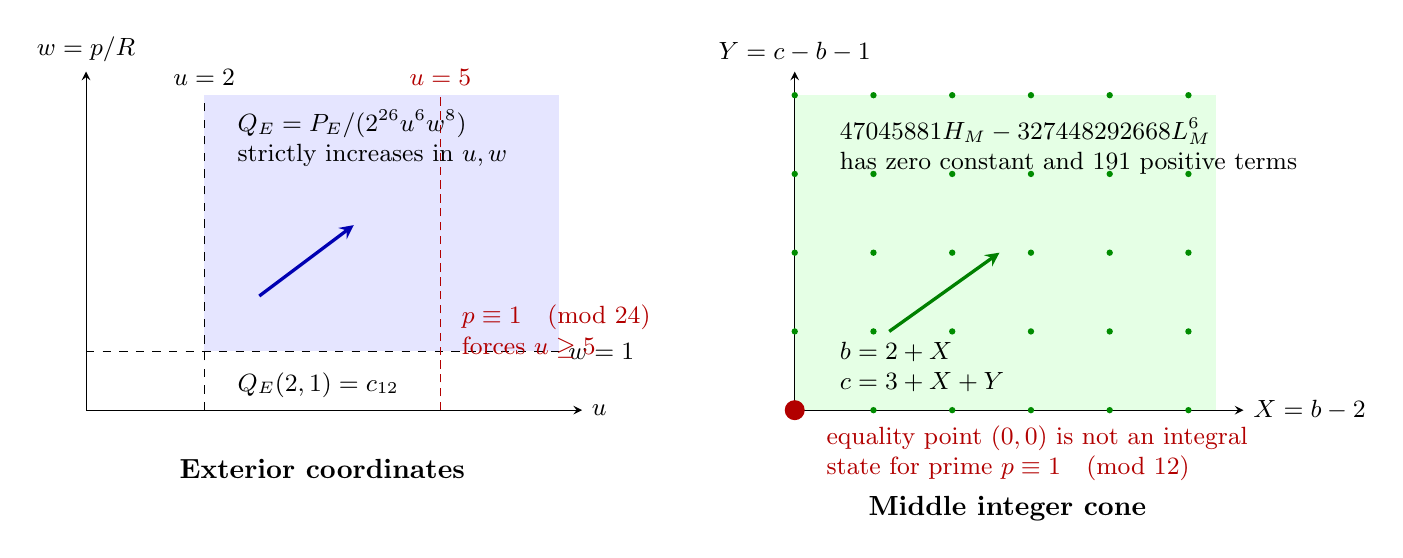
\begin{tikzpicture}[font=\small,>=stealth]
  % Exterior cone.
  \begin{scope}[xshift=0cm]
    \draw[->] (0,0) -- (6.3,0) node[right] {$u$};
    \draw[->] (0,0) -- (0,4.3) node[above] {$w=p/R$};
    \fill[blue!10] (1.5,0.75) rectangle (6,4);
    \draw[dashed] (0,0.75) -- (6,0.75) node[right] {$w=1$};
    \draw[dashed] (1.5,0) -- (1.5,4) node[above] {$u=2$};
    \draw[densely dashed,red!70!black] (4.5,0) -- (4.5,4) node[above] {$u=5$};
    \draw[->,very thick,blue!70!black] (2.2,1.45) -- (3.4,2.35);
    \node[align=left,anchor=west] at (1.8,3.45)
      {$Q_E=P_E/(2^{26}u^6w^8)$\\strictly increases in $u,w$};
    \node[align=left,anchor=west] at (1.8,0.32)
      {$Q_E(2,1)=c_{12}$};
    \node[align=left,anchor=west,red!70!black] at (4.65,1.0)
      {$p\equiv1\pmod{24}$\\forces $u\ge5$};
    \node[font=\bfseries] at (3,-0.75) {Exterior coordinates};
  \end{scope}

  % Middle cone.
  \begin{scope}[xshift=9cm]
    \draw[->] (0,0) -- (5.7,0) node[right] {$X=b-2$};
    \draw[->] (0,0) -- (0,4.3) node[above] {$Y=c-b-1$};
    \fill[green!10] (0,0) rectangle (5.35,4);
    \foreach \x in {0,...,5}{\foreach \y in {0,...,4}{\fill[green!55!black] (\x,\y) circle (1.15pt);}}
    \draw[->,very thick,green!50!black] (1.2,1.0) -- (2.6,2.0);
    \draw[fill=white,very thick,red!70!black] (0,0) circle (3pt);
    \node[align=left,anchor=west] at (0.45,3.35)
      {$47045881H_M-327448292668L_M^6$\\has zero constant and $191$ positive terms};
    \node[align=left,anchor=west] at (0.45,0.55)
      {$b=2+X$\\$c=3+X+Y$};
    \node[align=left,anchor=west,red!70!black] at (0.28,-0.55)
      {equality point $(0,0)$ is not an integral\\state for prime $p\equiv1\pmod{12}$};
    \node[font=\bfseries] at (2.7,-1.25) {Middle integer cone};
  \end{scope}
\end{tikzpicture}
}%
\caption{The two exact coordinate domains used in the global sign proof.  The
blue and green regions are certificate domains; actual Erd\H{o}s--Straus
witnesses are the arithmetic points satisfying the displayed gates and
integrality conditions.  The exterior lower bound is approached at the dashed
boundary $w=1$, which is excluded by $R<p$.  The middle comparison is strict at
every admissible lattice point because its only equality point would require
$a=6p/19$.}
\label{fig:coordinate-domains}
\end{figure}


\section{The original inverse, signs, norms, and conductor composition}
Let $\mathsf C_H$ be the displayed coefficient matrix of the four original
component polynomials and put
\[
 U_{nj}=\ell_j^n\xi_j,\qquad 0\le n,j\le3.
\]
Then $O,\mathsf C_H,U\in M_4(\mathbb C)$ and
\[
 O=\mathsf C_H U,\qquad
 \det\mathsf C_H=4F/A,\qquad \det U=\epsilon/A^2.
\]
For given $z=O\beta$, compute $m=\mathsf C_H^{-1}z$ by its actual adjugate and
determinant. The complete signed inverse is
\begin{align}\label{eq:inverse}
 \beta_j=\xi_j\bigl[&(C+B\ell_j+\ell_j^2+A\ell_j^3)m_0
 +(B+\ell_j+A\ell_j^2)m_1\notag\\
 &+(1+A\ell_j)m_2+A m_3\bigr].
\end{align}
This is Lagrange interpolation; $1/(\xi_jd_j)=\xi_j$. Its source comprises the
literal root labels and their retained signs. Neither squared norms nor an
unordered root list is asserted to reconstruct that source.

Here and in Theorem~\ref{thm:main}, $\|\cdot\|_2$ is the operator norm for the
standard Hermitian norm on $\mathbb C^4$. For four distinct positive integer
literal roots,
\[
 2/S\le |d_j|\le S^2.
\]
Indeed $|d_j|=S^{-1}\prod_{k\ne j}|\ell_j-\ell_k|$. The three nonzero integer
differences cannot all have magnitude one, while each is strictly less than
$S$.
The four row-entry bounds of $O$ are therefore
\[
 \sqrt{S/2},\qquad S,\qquad3S^2,\qquad20S^3.
\]
Every $3\times3$ cofactor has magnitude at most $360S^6$. The Frobenius norm of
the sixteen-cofactor adjugate is at most $1440S^6$. Dividing by the determinant
lower bound proves the inverse bound in Theorem~\ref{thm:main}.
For original positive label and receiving metrics $G$ and $Q$, respectively,
\begin{equation}\label{eq:metric}
 \|O^{-1}\|_{Q\to G}
 <\|G^{1/2}\|_2\|Q^{-1/2}\|_2\,
       \frac{360S^9}{c\,p^8}.
\end{equation}
No new invariant metric is substituted. If a further original linear observation
$\Lambda$ is retained, then
\[
 \ker(\Lambda O)=O^{-1}\ker\Lambda,\qquad
 \operatorname{rank}(\Lambda O)=\operatorname{rank}\Lambda.
\]
The receiver adds no further kernel on this arithmetic domain; it does not
assert that the observation itself is injective. On the image, for original
label metric $G$, its quotient metric is exactly
$(\Lambda O G^{-1}O^*\Lambda^*)^{-1}$. Transporting by $O$ uses
$O^{-*}GO^{-1}$ rather than assigning a new norm.
For an original invertible conductor
$L$, the complete inverse remains $(LO)^{-1}=O^{-1}L^{-1}$ with its actual
second factor. An enlarged receiving map
$\mathcal J(\alpha,\beta)=(\alpha,E\alpha+O\beta)$ likewise has the literal
inverse $(\alpha,z)\mapsto(\alpha,O^{-1}(z-E\alpha))$.

There is also a bound depending only on the prescribed prime. Let
\[
 s_p=p(p+3)/4,\qquad B_p=p+s_p(s_p+1).
\]
The tail factor identity bounds either tail by $pa(pa+1)/R$. Direct subtraction
from its value at $R=3$ gives
\[
 \frac{pa(pa+1)}R-\frac{s_p(s_p+1)}3
 =\frac{p^2(R-3)}{16}
   \left(1-\frac{p^2+4}{3R}\right)\le0.
\]
Since $a$ is smallest, $S\le B_p$. Thus \eqref{eq:metric} gives the explicit
coefficient bound $360B_p^9/(c\,p^8)=O(p^{28})$. It is a bound on every existing
integral witness, not an assertion that one exists. Homogeneous scaling gives
$\mathfrak N_p=p^8\mathfrak N_1$ and, with coherent signs,
$O_p=\operatorname{diag}(p^{-1},p,p^2,p^3)O_1$; these scale factors are retained.

\section{Arithmetic examples and precise nonclaims}
At the hard prime $p=1009$, the word $u=11$ at $a=253,R=3$ gives
\[
 E:(253,87032,3818056),\qquad
 M:(253,2042216,88792).
\]
The audit's character triple is $(-1,1,1)$ at this prime. The present theorem
nevertheless proves nonvanishing for every one of its integral witnesses.
For these two states $v_p(\mathfrak N)$ is respectively zero and two. At
$p=944329$, the original M state $(a,R,u)=(236094,47,1444)$ returns
\[
 (236094,780326438241,4772638766).
\]
All three old characters are positive, while the new negative bound still holds.
The exact integer numerators and original factor boxes appear in the certificate.

The theorem is not a claim that $\mathfrak N$ is a unit at $p$. In the complete
census over primes $p\equiv1\pmod{12}$ through $3000$, the valuation histogram
is $E:v_p=0$ for $2447$ states, $E:v_p=1$ for four states, and $M:v_p=2$ for
$2054$ states. The arithmetic order/conductor defects studied earlier remain;
nonvanishing over $\mathbb Q$ is a different assertion.

A positive real counterdomain also remains. For $3\le t\le4$, put
\[
 p=1,\quad b=t,\quad c=t+1/10,\quad a=bc/(4bc-b-c).
\]
These are distinct positive reciprocal roots with $1/4<a<1/2<1<t<t+1/10$.
Put $D=40t^2-16t-1$. Exact elimination gives
\[
 \mathfrak N(t)=\frac{P(t)}{100000D^6},
\]
where, in descending order from $t^{18}$ to the constant term, the coefficient
vector of $P$ is
\[
\begin{gathered}
(3617792000000000,-26154803200000000,70130040320000000,\\
-88735357952000000,45725157043200000,12437702609920000,\\
-28537312234432000,13617485725683200,-1729738000411520,\\
-478292746960768,90264805813440,17381353732960,-951549897144,\\
-455951154664,-51247817566,-3092472120,-110106797,-2195730,-19035).
\end{gathered}
\]
All eighteen coefficients of $P'(3+X)$ are positive. Exact endpoint signs
therefore give a unique receiver singularity
\[
 \frac{3053}{1000}<t_0<\frac{1527}{500},
 \qquad t_0\approx3.05367681075890,
\]
while the quartic remains squarefree. The M separation
$c-b\ge1$ fails. The E raw word is also below one at both endpoints. Scaling
by any prime $p>5$ leaves the tail gap $p/10$ nonintegral, so these points cannot
be promoted to integral witnesses. The audit's separate positive-real example
and $p$-adic zeros are not contradicted by Theorem~\ref{thm:main}.

Finally, even an available divisor need not satisfy a gate. At $p=1009,a=321$,
$R=275,u=9$, the raw exterior identity is
\[
 (321,335338/275,9486618/275).
\]
Its rational quantity $S^6F$ is strictly negative by Lemma~\ref{lem:Epoly}, but
$275\nmid37$: the E divisibility gate fails. Frame invertibility therefore does not force an original
integer coefficient. The divisor-descent handoff's universal occupancy
obligation is unchanged \cite{Descent}.

\section{Certificate scope and reproducibility}
Run the two separate implementations with the stated bounds:
\begin{verbatim}
python verify.py --bound 3000 --out certificates
python -O verify.py --bound 3000 --out certificates_optimized
python check_independent.py --input certificates \
  --out certificates/independent.json
\end{verbatim}
The first program performs the universal Laurent-polynomial reduction, all
coefficient identities and the original divisor scan. The second uses the
unexpanded supplied $F$, complete unisolvent grids, separate binomial arithmetic,
and a primitive $(h,r,s)$ enumeration. It imports neither the first program nor
predecessor software. Both use only the Python standard library and explicit
checks that remain present under optimized execution.

The bounded arithmetic lane covers every first-half source at primes
$p\equiv1\pmod{12}$ through 3000: 99 primes, 34287 shells, 868359 original
divisor words, 2451 E states and 2054 oriented M states. Source hashes,
execution outcomes and negative-control values are recorded separately.
This is not a new overall ES verification range, an independent mathematical
review, or a Lean build. The universal theorem is the proved arithmetic
reduction together with the complete polynomial certificates.

The precise newly closed question is nonvanishing of the supplied odd
receiving determinant at every positive integral hard-prime witness. The
initial existence of such a witness is not a premise that can be discharged
by this nonvanishing theorem. The work remains at the programme's Turn~7.

\appendix
\section{Compact coefficient ledger}
The full arrays are machine-readable; the following minima make their signs
visible without replacing the identity checks.
\begin{table}[htbp]
\centering\scriptsize
\caption{Exterior coefficient minima. Each row contains 17 coefficients in each of the three arrays.}\label{tab:E}
\begin{tabular}{r r r r}
\toprule
$X$ degree & $P_E(1+X,1+Y)$ & $uP_{E,u}-6P_E$ shifted & $wP_{E,w}-8P_E$ shifted\\
\midrule
0 & 414843750 & 1950703125 & 3318750000\\
1 & 4439765625 & 21170421875 & 35518125000\\
2 & 21684625000 & 105062450000 & 173477000000\\
3 & 63933650000 & 315267850000 & 511469200000\\
4 & 126767200000 & 637111680000 & 1014137600000\\
5 & 178129216000 & 913469734400 & 1425033728000\\
6 & 181933158400 & 952827043840 & 1455465267200\\
7 & 136118149120 & 728564637696 & 1088945192960\\
8 & 74055811072 & 405315584000 & 592446488576\\
9 & 28578217984 & 160000049152 & 228625743872\\
10 & 7426539520 & 42543874048 & 59412316160\\
11 & 1167065088 & 6841958400 & 9336520704\\
12 & 83886080 & 503316480 & 671088640\\
\bottomrule
\end{tabular}
\end{table}
\begin{table}[htbp]
\centering\small
\caption{Middle comparison polynomial: every nonzero coefficient is positive; its constant is zero.}\label{tab:M}
\begin{tabular}{r r r}
\toprule
$Y$ degree & Nonzero count & Minimum coefficient\\
\midrule
0 & 18 & 12224401719040\\
1 & 19 & 28134189572096\\
2 & 19 & 14067094786048\\
3 & 18 & 126603853074432\\
4 & 17 & 510269410869248\\
5 & 16 & 1212467950600192\\
6 & 15 & 1880365903044608\\
7 & 14 & 1988277863047168\\
8 & 13 & 1451415862034432\\
9 & 12 & 722239332302848\\
10 & 11 & 234515813076992\\
11 & 10 & 44899083358208\\
12 & 9 & 3853998571520\\
\bottomrule
\end{tabular}
\end{table}

